\documentclass[10pt]{article}
\usepackage{icmlko}

\icmlmeta{IP 파운데이션 월드모델}{146}{결정적이라고 적혀 있던 스무 노트}{노트 145가 ``다른 가드도 극값 통계를 쓰고 있나''를 남겼다. 있었다 --- 그런데 그 가드의 더 큰 문제는 극값이 아니라 재는 시늉만 하고 있었다는 것이다}

\begin{document}

\twocolumn[
\icmlheader

\begin{abstract}
가드 열하나를 훑었다. 극값을 쓰는 것은 둘 --- 재현(씨앗 넷의 최대$-$최소)과
묶음(최대 묶음 크기)이다. 묶음은 정당하다(재는 대상 자체가 최대 묶음이다).
재현을 들여다보다 \textbf{극값보다 큰 것을 찾았다.} 그 가드는 씨앗을 바꾸려고
\texttt{np.random.seed(s)}를 부르는데, 이 판의 정식화는 전부 생성자에서 받은
씨앗으로 \texttt{np.random.default\_rng} 를 만든다. \textbf{전역 씨앗은
아무것도 안 바꿨다.} 그래서 스무 노트 동안 모든 정식화가 ``씨앗 넷 폭
0.0000''으로 --- 즉 결정적이라고 --- 보고됐다. 실제로 재 보니 F18 배깅은
팝업 $\rho$가 씨앗에 \textbf{0.0590} 움직이고 F8 부스팅은 0.0266, F9는
0.0148이다. 고쳤다. 겸사겸사 판정도 극값에서 예측 자기상관으로 바꿨다 ---
$k$개 표본의 범위는 기대값이 $k$와 함께 커지므로($d_2{=}1.13$,
$d_4{=}2.06$), 예산 안에서 두 번만 돈 비싼 정식화가 자동으로 유리했다.
\textbf{그리고 순위표를 다시 봤다.} 판 $\rho$의 씨앗 표준편차가 F8에서
0.0047, 두 정식화 차이의 짝 표준편차가 0.0087이다. 순위표 상위 열셋의
\textbf{연속 격차 열둘 중 열이 그 값보다 작다.} 위 여섯은 순위가 없는 것과
같다. \textbf{노트 145도 고친다} --- 거기서 ``판 $\rho$''로 나란히 적은 두
표가 사실 다른 통계였다(문턱 40은 단순 평균, 문턱 15는 순위 지표). 순위
지표로 통일하면 문턱 40의 배깅 이득이 $+$0.0185가 아니라 \textbf{$+$0.0063
$\pm$ 0.0087}이다. 노트 145의 결론(``채택 근거는 점수가 아니라 귀착이다'')은
그대로고, 오히려 더 맞다 --- 점수 이득은 어느 설정에도 없다.
\end{abstract}
]

\begin{figure*}[t]
\centering
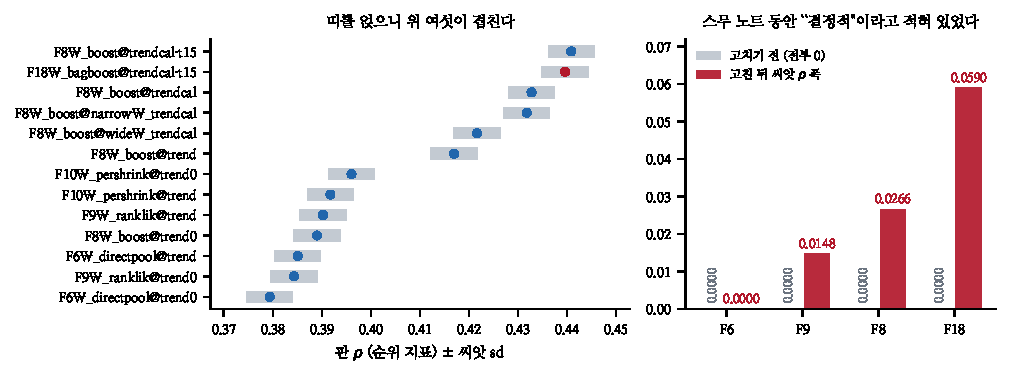
\includegraphics[width=\textwidth]{figs/seed.pdf}
\caption{왼쪽 --- 씨앗 띠를 얹은 순위표. 오른쪽 --- 고치기 전 재현 가드는
전부 0을 보고했다.}
\end{figure*}

\section{가드 열하나를 훑었다}

\begin{table}[t]
\centering\tsize
\caption{가드가 쓰는 통계.}
\begin{tabular}{lll}
\toprule
& 통계 & 판정 \\
\midrule
치환 & $R{=}99$ 귀무 & 괜찮다 (노트 125에서 고침) \\
분해능 & 붓스트랩 400 백분위 & 괜찮다 \\
집단 & 평균 · 모의 보정 & 괜찮다 (노트 137) \\
평탄 & 단일 적합 사분위 & 반복이 아니라 괜찮다 \\
묶음 & \textbf{최대} 묶음 & 재는 대상이 최대다 \\
\textbf{재현} & \textbf{씨앗 넷 최대$-$최소} & \textbf{고쳐야 한다} \\
\bottomrule
\end{tabular}
\end{table}

\claimx{\textbf{극값을 쓰는 것은 둘뿐이고 하나는 정당하다.} 묶음 가드가
재는 것은 ``같은 값에 뭉친 제일 큰 덩어리''이므로 최대가 곧 대상이다.
재현만 남는다.}{노트 145의 걱정이 절반은 기우였다. 다만 남은 하나가
컸다.}

\section{재는 시늉만 하고 있었다}

\begin{table}[t]
\centering\tsize
\caption{팝업 $\rho$. 씨앗 넷.}
\begin{tabular}{lrr}
\toprule
& 고치기 전 & \textbf{고친 뒤} \\
\midrule
F6 능형 & .0000 & .0000 (진짜 결정적) \\
F9 순위우도 & .0000 & \textbf{.0148} \\
F8 부스팅 & .0000 & \textbf{.0266} \\
F18 배깅 & .0000 & \textbf{.0590} \\
\bottomrule
\end{tabular}
\end{table}

\claimx{\textbf{전역 씨앗은 아무것도 안 바꿨다.} 가드는
\texttt{np.random.seed(s)}를 부르는데 정식화는 \texttt{default\_rng(self.seed)}
를 쓴다 --- 두 난수원은 서로 모른다. 이제 객체의 씨앗 속성을 직접 갈아
끼운다.}{F6 능형만 진짜로 결정적이다. 나머지 셋은 스무 노트 동안 ``씨앗
넷 폭 0.0000''을 달고 채택 심사를 통과했다.}

\claimx{\textbf{판정도 극값에서 자기상관으로 바꿨다.} $k$개 표본의 범위는
기대값이 $k$와 함께 커진다. 예산 안에서 두 번만 도는 비싼 정식화가 네 번
도는 싼 것보다 자동으로 좁게 나왔다 --- 비쌀수록 유리한 판정이었다.}{자기상관은
라벨을 안 본다. 귀착 가드(노트 144 · 145)와 같은 통계이고, 둘의 차이는
무엇을 흔드느냐뿐이다 --- 재현은 씨앗, 귀착은 풀.}

\section{순위표에 띠를 얹으면}

\begin{table}[t]
\centering\tsize
\caption{판 $\rho$의 씨앗 흔들림. 문턱 40 · 검색$+$달력, 씨앗 다섯.}
\begin{tabular}{lrr}
\toprule
& 평균 & sd \\
\midrule
F8 부스팅 & $+$.4281 & .0047 \\
F18 배깅 & $+$.4345 & .0063 \\
\midrule
\textbf{차} & \textbf{$+$.0063} & \textbf{.0087} \\
\bottomrule
\end{tabular}
\end{table}

\claimx{\textbf{순위표 위 여섯은 순위가 없다.} 상위 열셋의 연속 격차 열둘
중 열이 짝 표준편차 0.0087보다 작다. 1위와 2위의 격차는 0.0013이고 그것은
씨앗을 바꾸면 뒤집힌다.}{판 $\rho$ 자체가 여러 대상의 가중 평균이라 개별
대상보다는 안정적이다. 그래도 이 정도다.}

이제 실행마다 씨앗 흔들림과 귀착 자기상관을 요약에 같이 싣는다. 순위표에
띠가 없으면 순위가 해상도를 넘어서 읽힌다.

\section{노트 145를 고친다}

노트 145의 두 표에 ``판 $\rho$''라고 나란히 적었는데 서로 다른 통계였다 ---
문턱 40 표는 대상 평균(\texttt{board}), 문턱 15 표는 순위 지표
(\texttt{pooled})다. 순위 지표는 노트 126 이후 이 판의 판정치이므로 그것으로
통일한다.

\begin{table}[t]
\centering\tsize
\caption{배깅 대 부스팅. 순위 지표로 통일.}
\begin{tabular}{lrr}
\toprule
& 노트 145가 적은 값 & \textbf{순위 지표} \\
\midrule
문턱 40 & $+$.0185 (평균) & \textbf{$+$.0063 $\pm$ .0087} \\
문턱 15 & $-$.0013 & $-$.0013 \\
\bottomrule
\end{tabular}
\end{table}

\claimx{\textbf{점수 이득은 어느 설정에도 없다.} 노트 145는 ``문턱 40에서는
오르고 15에서는 안 오른다''로 읽었는데, 순위 지표로 보면 40에서도 안 오른다.
결론(``채택 근거는 점수가 아니라 귀착이다'')은 그대로이고 더 깨끗해진다.}{배깅의
귀착 이득(0.906 → 0.948)은 그대로다 --- 그 값은 라벨을 안 보므로 이 정정에
안 걸린다.}

\begin{table}[t]
\centering\tsize
\caption{남은 것.}
\begin{tabular}{ll}
\toprule
순위표 & 위 여섯이 겹친다 --- 가르려면 표본이 필요하다 \\
씨앗 & 채택 문턱 0.05 는 어디서 왔나 --- 교정 안 됨 \\
비용 & 배깅은 여덟 배인데 사는 것이 귀착뿐이다 \\
\bottomrule
\end{tabular}
\end{table}

첫 줄이 다음 자리다. 순위표를 가르는 길은 두 가지뿐이다 --- 대상을 늘리거나
(팝업 59건이 병목이고 노트 132가 상한을 202로 쟀다), 판정치의 분산을 줄이거나.
후자는 방법 문제이고, 씨앗 평균을 판정치로 쓰는 것부터가 그 한 수다.

\end{document}
